\begin{task}[credit=4]{\codesym~Zufallswälder}
In dieser Aufgabe verwenden wir den PtU Datensatz (s. Abb.~\ref{fig:shearcutting}), um mit einem Zufallswald (engl. Random Forest) die Geschwindigkeit des Einschlags aus den Zeitreihen zu klassifizieren.
 
\begin{subtask}[points=2,title=\codesym~\texttt{04\_random\_forest.py}]
Laden Sie die Daten des Kraftsensor aus \texttt{Filename\_Fz\_raw.csv} und die Geschwindigkeit des Stanzen aus \texttt{Filename\_Speed.csv} und vervollständigen Sie den Code in \texttt{04\_random\_forest.py}:

\begin{itemize}
\item[\codesym] Trainieren Sie einen Zufallswald aus $100$ Entscheidungsstümpfen in der Methode \texttt{fit\_tree\_stump\_forest()}.

\item[\codesym] Trainieren Sie einen einzelnen Entscheidungsstumpf in der Methode \texttt{fit\_tree\_stump()}.
\end{itemize}
\end{subtask}

\begin{subtask}[title=Konfusionsmatrix,points=2]
Geben Sie die Konfusionsmatrizen des Trainings- und Testdatensatzes mit absoluten Werten für den Zufallswald  an.

\begin{solution}
	Es ergab sich für den Trainingsdatensatz die confusion matrix:
		\begin{table}[H]
			\begin{tabular}{lll}
				658 & 0   & 0   \\
				0   & 831 & 0   \\
				11  & 6   & 723
			\end{tabular}
		\end{table}
	und für den Testdatensatz:
		\begin{table}[H]
			\begin{tabular}{lll}
				166 & 0   & 0   \\
				0   & 207 & 0   \\
				2   & 4   & 179
			\end{tabular}
		\end{table}
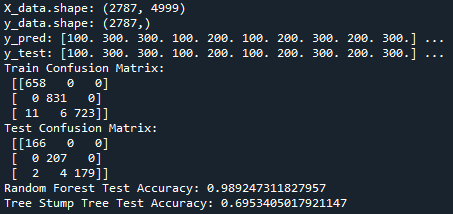
\includegraphics[width=\linewidth]{ue4ergebnisse.png}
\end{solution}

\end{subtask}

\end{task}
